\chapter{ACTUAL WORK}

\section{Methodology for the Study}

The research methodology follows a systematic, objective-driven approach to build an end-to-end DoS detection and mitigation system. The study is structured into four sequential objectives, each building upon the output of the previous one, culminating in a complete pipeline that transforms raw network traffic features into actionable security responses.

\subsection{Research Design}

The research adopts an experimental design comprising four phases: (1)~data preparation and feature engineering, (2)~comparative machine learning model training and selection, (3)~integration of Explainable AI for model transparency, and (4)~development of a rule-based mitigation framework driven by XAI outputs. The overall system architecture is illustrated in Figure~\ref{fig:system_architecture}.

\begin{figure}[htbp]
    \centering
    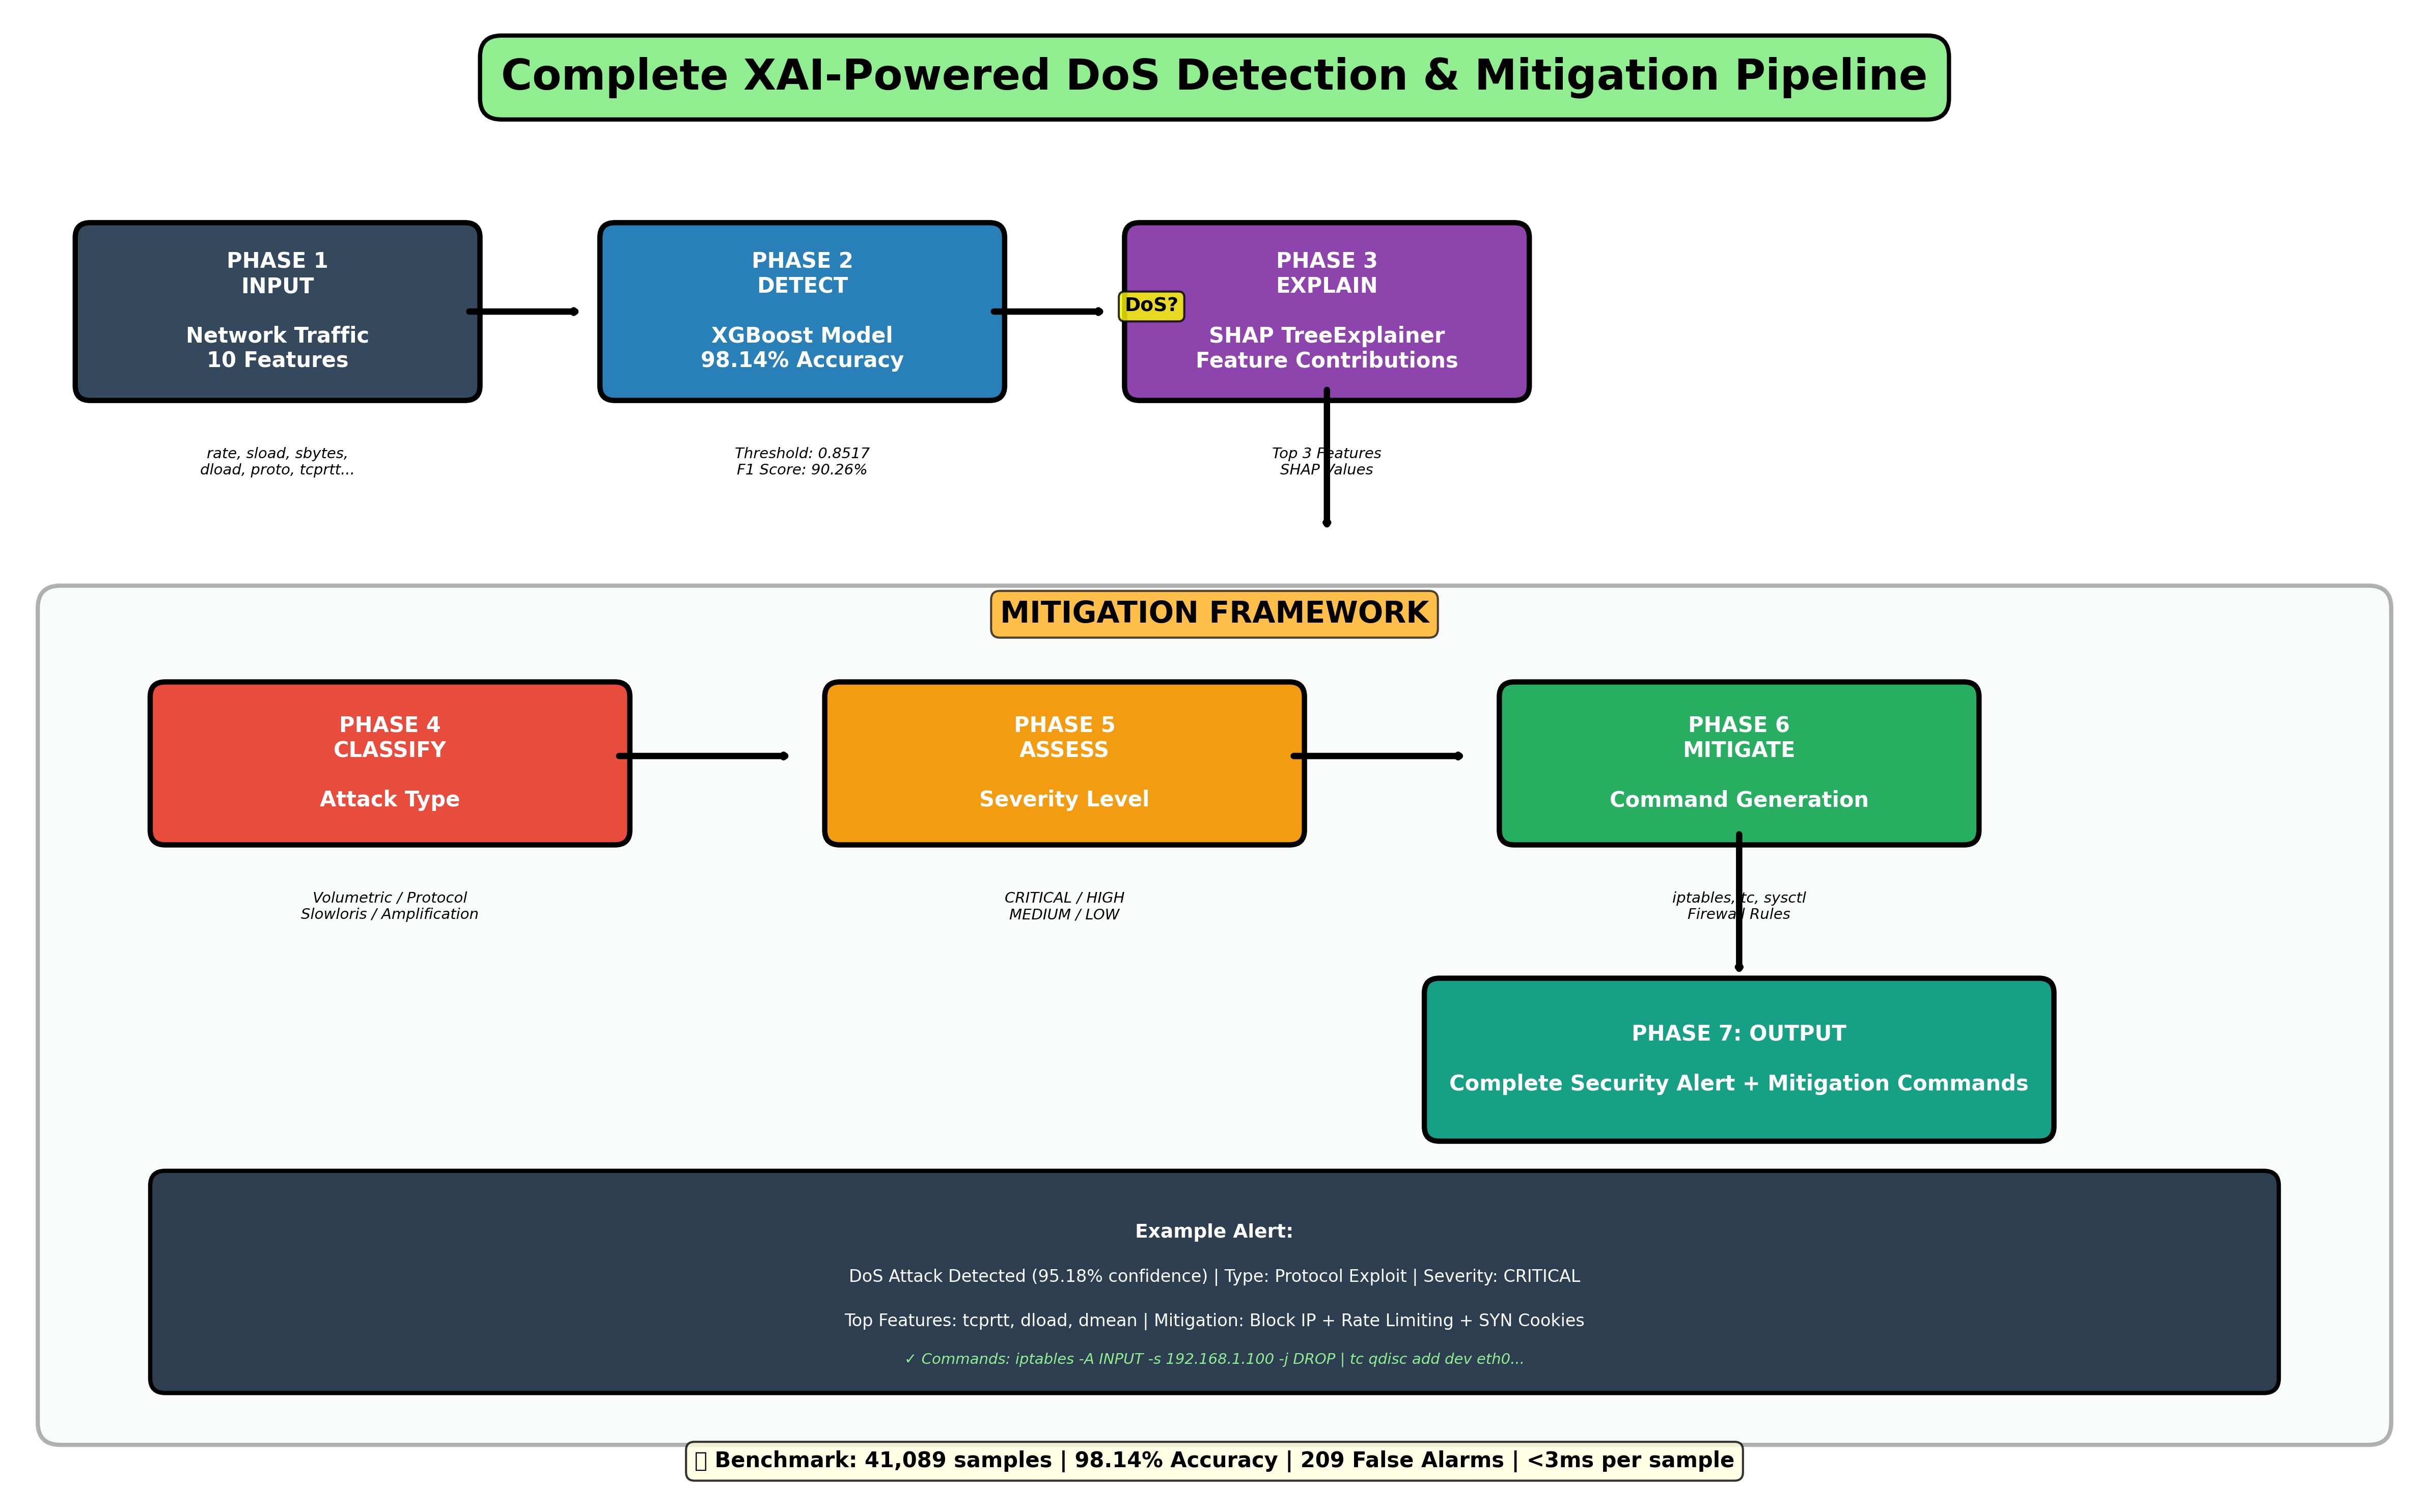
\includegraphics[width=0.95\textwidth]{presentation_diagrams/complete_pipeline_highlevel.png}
    \caption{High-level system architecture: Detection to Defense pipeline}
    \label{fig:system_architecture}
\end{figure}

\subsection{Dataset Selection}

The UNSW-NB15 dataset, developed by the University of New South Wales, was selected as the primary benchmark dataset. It is a widely recognised network intrusion detection dataset containing realistic modern network traffic with both normal and attack records. Table~\ref{tab:dataset_properties} summarises the key properties of the dataset.

\begin{table}[htbp]
    \centering
    \caption{UNSW-NB15 dataset properties}
    \label{tab:dataset_properties}
    \begin{tabular}{ll}
        \toprule
        \textbf{Property} & \textbf{Details} \\
        \midrule
        Source & University of New South Wales (UNSW) \\
        Total Records & 257,673 (175,341 training + 82,332 testing) \\
        Original Features & 49 columns \\
        Attack Categories & 10 types (DoS, Exploits, Fuzzers, Generic, etc.) \\
        Focus & Binary classification: DoS vs Normal \\
        \bottomrule
    \end{tabular}
\end{table}

\subsection{Data Splitting Strategy}

A critical aspect of the methodology is the use of \textbf{completely separate CSV files} for training and testing, as officially provided by the UNSW-NB15 authors. The model has never seen any testing data during training, constituting true external validation.

The training set was balanced to 24,528 samples (12,264~DoS + 12,264~Normal) by random undersampling of the majority class. This ensures equal class representation during training and prevents the model from developing bias towards normal traffic. The testing set was kept at its natural imbalanced ratio of approximately 90\%~normal and 10\%~DoS (37,000~normal + 4,089~DoS = 41,089~total), simulating realistic network conditions where attacks are rare events. The class distributions of both sets are shown in Figure~\ref{fig:data_distribution}.

\begin{figure}[htbp]
    \centering
    \begin{subfigure}[b]{0.48\textwidth}
        \centering
        \includegraphics[width=\textwidth]{03_model_training/proper_training/images/02_training_set_distribution.png}
        \caption{Training set (balanced 50/50)}
    \end{subfigure}
    \hfill
    \begin{subfigure}[b]{0.48\textwidth}
        \centering
        \includegraphics[width=\textwidth]{03_model_training/proper_training/images/01_testing_set_distribution.png}
        \caption{Testing set (imbalanced 90/10)}
    \end{subfigure}
    \caption{Class distribution of training and testing datasets}
    \label{fig:data_distribution}
\end{figure}

\subsection{Feature Engineering}

From the original 49~columns in the UNSW-NB15 dataset, 10~features were selected based on a combination of correlation analysis, variance analysis, preliminary model feature importance scores, and domain knowledge of DoS attack characteristics. Table~\ref{tab:features} describes each selected feature and its relevance to DoS detection.

\begin{table}[htbp]
    \centering
    \caption{Selected features and their DoS relevance}
    \label{tab:features}
    \begin{tabular}{clll}
        \toprule
        \textbf{\#} & \textbf{Feature} & \textbf{Description} & \textbf{DoS Relevance} \\
        \midrule
        1  & \texttt{rate}   & Packets per second          & DoS floods spike packet rate \\
        2  & \texttt{sload}  & Source bits/sec              & High sload indicates flood \\
        3  & \texttt{sbytes} & Source-to-dest bytes         & Excessive data transfer \\
        4  & \texttt{dload}  & Destination bits/sec         & High in amplification attacks \\
        5  & \texttt{proto}  & Network protocol (encoded)   & Protocol-specific attacks \\
        6  & \texttt{dtcpb}  & Dest TCP base sequence \#    & SYN flood indicator \\
        7  & \texttt{stcpb}  & Source TCP base sequence \#   & SYN flood indicator \\
        8  & \texttt{dmean}  & Dest packet mean size        & Small in floods, large in slowloris \\
        9  & \texttt{tcprtt} & TCP round-trip time           & Increases under DoS load \\
        10 & \texttt{dur}    & Connection duration           & Long in slowloris attacks \\
        \bottomrule
    \end{tabular}
\end{table}

The preprocessing pipeline consists of three steps: (1)~\textbf{Protocol Encoding} using \texttt{LabelEncoder} to convert the categorical \texttt{proto} column into numeric values (132~classes; \texttt{tcp}$\rightarrow$112, \texttt{udp}$\rightarrow$118), (2)~\textbf{Feature Scaling} using \texttt{StandardScaler} to normalise all features to zero mean and unit variance, fitted exclusively on the training data to prevent data leakage, and (3)~\textbf{Missing Value Imputation} using column median values. The fitted scaler and encoder are persisted as \texttt{.pkl} files for reproducible inference.

%----------------------------------------------------------------------
\section{Experimental and/or Analytical Work Completed in the Project}

\subsection{Comparative Model Training}

Eight machine learning models were trained and evaluated, spanning classical algorithms, ensemble methods, shallow neural networks, and deep learning architectures. All models were trained on the same balanced training set (24,528~samples) and evaluated on the same imbalanced external test set (41,089~samples). Table~\ref{tab:models_trained} lists the models and their categories.

\begin{table}[htbp]
    \centering
    \caption{Machine learning models trained and evaluated}
    \label{tab:models_trained}
    \begin{tabular}{clll}
        \toprule
        \textbf{\#} & \textbf{Model} & \textbf{Type} & \textbf{Category} \\
        \midrule
        1 & XGBoost              & Gradient Boosting           & Ensemble \\
        2 & Random Forest         & Bagging Ensemble            & Ensemble \\
        3 & Decision Tree         & Single Tree Classifier      & Classical \\
        4 & MLP                   & Multi-Layer Perceptron      & Shallow Neural Network \\
        5 & SVM                   & Support Vector Machine      & Classical \\
        6 & Logistic Regression   & Linear Classifier           & Classical (Baseline) \\
        7 & LSTM                  & Long Short-Term Memory      & Deep Learning (Recurrent) \\
        8 & 1D-CNN                & 1D Convolutional Network    & Deep Learning (Convolutional) \\
        \bottomrule
    \end{tabular}
\end{table}

For the classical and ensemble models, 5-fold stratified cross-validation was used during training to estimate generalisation performance. Table~\ref{tab:cv_results} presents the cross-validation results.

\begin{table}[htbp]
    \centering
    \caption{5-Fold stratified cross-validation results on training set}
    \label{tab:cv_results}
    \begin{tabular}{lcccc}
        \toprule
        \textbf{Model} & \textbf{CV Accuracy} & \textbf{CV Precision} & \textbf{CV Recall} & \textbf{CV F1} \\
        \midrule
        XGBoost             & 96.45\% $\pm$0.42 & 96.89\% $\pm$0.52 & 95.95\% $\pm$0.58 & 96.45\% $\pm$0.42 \\
        Random Forest       & 96.22\% $\pm$0.38 & 96.75\% $\pm$0.48 & 95.63\% $\pm$0.62 & 96.22\% $\pm$0.38 \\
        Decision Tree       & 95.55\% $\pm$1.39 & 96.84\% $\pm$1.30 & 94.18\% $\pm$3.42 & 95.48\% $\pm$1.50 \\
        MLP                 & 94.32\% $\pm$0.60 & 95.38\% $\pm$0.72 & 93.02\% $\pm$0.88 & 94.32\% $\pm$0.60 \\
        SVM                 & 92.26\% $\pm$0.75 & 93.45\% $\pm$0.85 & 90.88\% $\pm$1.02 & 92.26\% $\pm$0.75 \\
        Logistic Regression & 86.64\% $\pm$1.15 & 90.11\% $\pm$1.24 & 82.05\% $\pm$1.82 & 86.27\% $\pm$1.15 \\
        \bottomrule
    \end{tabular}
\end{table}

\subsection{Threshold Optimization}

A key analytical step was threshold optimisation. At the default classification threshold of 0.5, precision was low due to the 9:1 class imbalance in the test set---even a small false positive rate on 37,000~normal samples produces a large absolute number of false alarms. To address this, threshold optimisation was performed by searching over 100~candidate thresholds $[0.00, 0.01, \ldots, 1.00]$ and selecting the threshold that maximises the F1~score. Table~\ref{tab:optimized_results} presents the results at each model's optimised threshold.

\begin{table}[htbp]
    \centering
    \caption{External benchmark results at optimised thresholds (41,089 unseen samples)}
    \label{tab:optimized_results}
    \begin{tabular}{lcccccc}
        \toprule
        \textbf{Model} & \textbf{Acc.} & \textbf{Prec.} & \textbf{Recall} & \textbf{F1} & \textbf{Threshold} & \textbf{AUC} \\
        \midrule
        \textbf{XGBoost}    & \textbf{97.76\%} & \textbf{94.41\%} & \textbf{87.09\%} & \textbf{90.57\%} & \textbf{0.8517} & \textbf{0.9915} \\
        Random Forest       & 97.54\% & 94.44\% & 85.42\% & 89.70\% & 0.8333 & 0.9900 \\
        Decision Tree       & 97.83\% & 93.43\% & 84.13\% & 88.53\% & 0.93   & 0.9806 \\
        1D-CNN              & 97.42\% & 90.92\% & 82.27\% & 86.38\% & 0.87   & 0.9780 \\
        MLP                 & 97.14\% & 88.43\% & 82.02\% & 85.11\% & 0.8448 & 0.9753 \\
        LSTM                & 96.89\% & 88.12\% & 79.48\% & 83.58\% & 0.79   & 0.9683 \\
        SVM                 & 95.86\% & 82.47\% & 74.10\% & 78.06\% & 0.93   & --- \\
        Logistic Regression & 88.42\% & 44.48\% & 66.06\% & 53.16\% & 0.7468 & --- \\
        \bottomrule
    \end{tabular}
\end{table}

XGBoost achieved the highest F1~score (90.57\%), highest AUC~(0.9915), and the lowest false alarm rate (209~false positives out of 37,000~normal samples, i.e., 0.56\%). It was therefore selected as the production model. The cross-validation performance comparison is shown in Figure~\ref{fig:model_comparison}, and the confusion matrices for XGBoost on the training and testing sets are shown in Figure~\ref{fig:confusion_matrices}.

\begin{figure}[htbp]
    \centering
    \includegraphics[width=0.85\textwidth]{03_model_training/proper_training/images/03_model_performance_training.png}
    \caption{Model performance comparison during cross-validation}
    \label{fig:model_comparison}
\end{figure}

\begin{figure}[htbp]
    \centering
    \begin{subfigure}[b]{0.48\textwidth}
        \centering
        \includegraphics[width=\textwidth]{03_model_training/proper_training/images/04_xgboost_confusion_matrix_training.png}
        \caption{Training set confusion matrix}
    \end{subfigure}
    \hfill
    \begin{subfigure}[b]{0.48\textwidth}
        \centering
        \includegraphics[width=\textwidth]{03_model_training/proper_training/images/05_xgboost_confusion_matrix_testing.png}
        \caption{Testing set confusion matrix (threshold=0.8517)}
    \end{subfigure}
    \caption{XGBoost confusion matrices on training and external testing sets}
    \label{fig:confusion_matrices}
\end{figure}

\subsection{Why Deep Learning Models Performed Lower}

An important analytical finding is that the LSTM (F1:~83.58\%) and 1D-CNN (F1:~86.38\%) underperformed the tree-based ensemble models. This result is consistent with established machine learning literature. The UNSW-NB15 dataset provides pre-computed, engineered flow-level features in a tabular format. Tree-based models such as XGBoost are specifically optimised for tabular data and can exploit feature interactions efficiently through recursive partitioning. In contrast, LSTMs and CNNs are architecturally designed for raw sequential or spatial data (e.g., raw packet captures or images). When applied to pre-aggregated tabular features, their structural advantages---temporal memory for LSTMs and local pattern detection for CNNs---cannot be fully leveraged.

%----------------------------------------------------------------------
\section{Modeling, Analysis \& Design}

\subsection{XGBoost Model Configuration}

The selected XGBoost model was configured with the following hyperparameters: \texttt{n\_estimators}=100, \texttt{max\_depth}=6, \texttt{learning\_rate}=0.1, and \texttt{random\_state}=42. The model produces a probability score $P(\text{DoS}) \in [0, 1]$ for each input sample. At the optimised threshold of 0.8517, a sample is classified as a DoS attack if $P(\text{DoS}) \geq 0.8517$ and as normal traffic otherwise.

The XGBoost feature importance, shown in Figure~\ref{fig:feature_importance}, reveals that \texttt{sload} (source bandwidth), \texttt{rate} (packets per second), and \texttt{sbytes} (source bytes) are the top three discriminative features for DoS detection. This aligns with domain knowledge, as DoS attacks characteristically generate abnormally high traffic volumes and rates.

\begin{figure}[htbp]
    \centering
    \includegraphics[width=0.75\textwidth]{03_model_training/proper_training/images/06_xgboost_feature_importance.png}
    \caption{XGBoost feature importance ranking}
    \label{fig:feature_importance}
\end{figure}

\subsection{Explainable AI Design: SHAP TreeExplainer}

To provide transparency into the model's decision-making process, SHAP (SHapley Additive exPlanations) was integrated using the TreeExplainer algorithm. SHAP calculates a contribution score (SHAP~value) for each feature in every prediction, quantifying how much each feature pushed the prediction towards DoS or towards Normal. Positive SHAP values indicate a push towards the DoS class, while negative values push towards Normal. The sum of all SHAP values equals the model's log-odds output.

SHAP TreeExplainer was chosen over alternatives such as LIME because it provides \textbf{mathematically exact} Shapley values for tree-based models, is \textbf{deterministic} (same input always produces the same explanation), and is computationally efficient---running in seconds rather than minutes. Figure~\ref{fig:shap_summary} shows the global SHAP summary plot across 500 randomly sampled test records, while Figure~\ref{fig:shap_waterfall} illustrates per-record explanations for individual DoS and Normal predictions.

\begin{figure}[htbp]
    \centering
    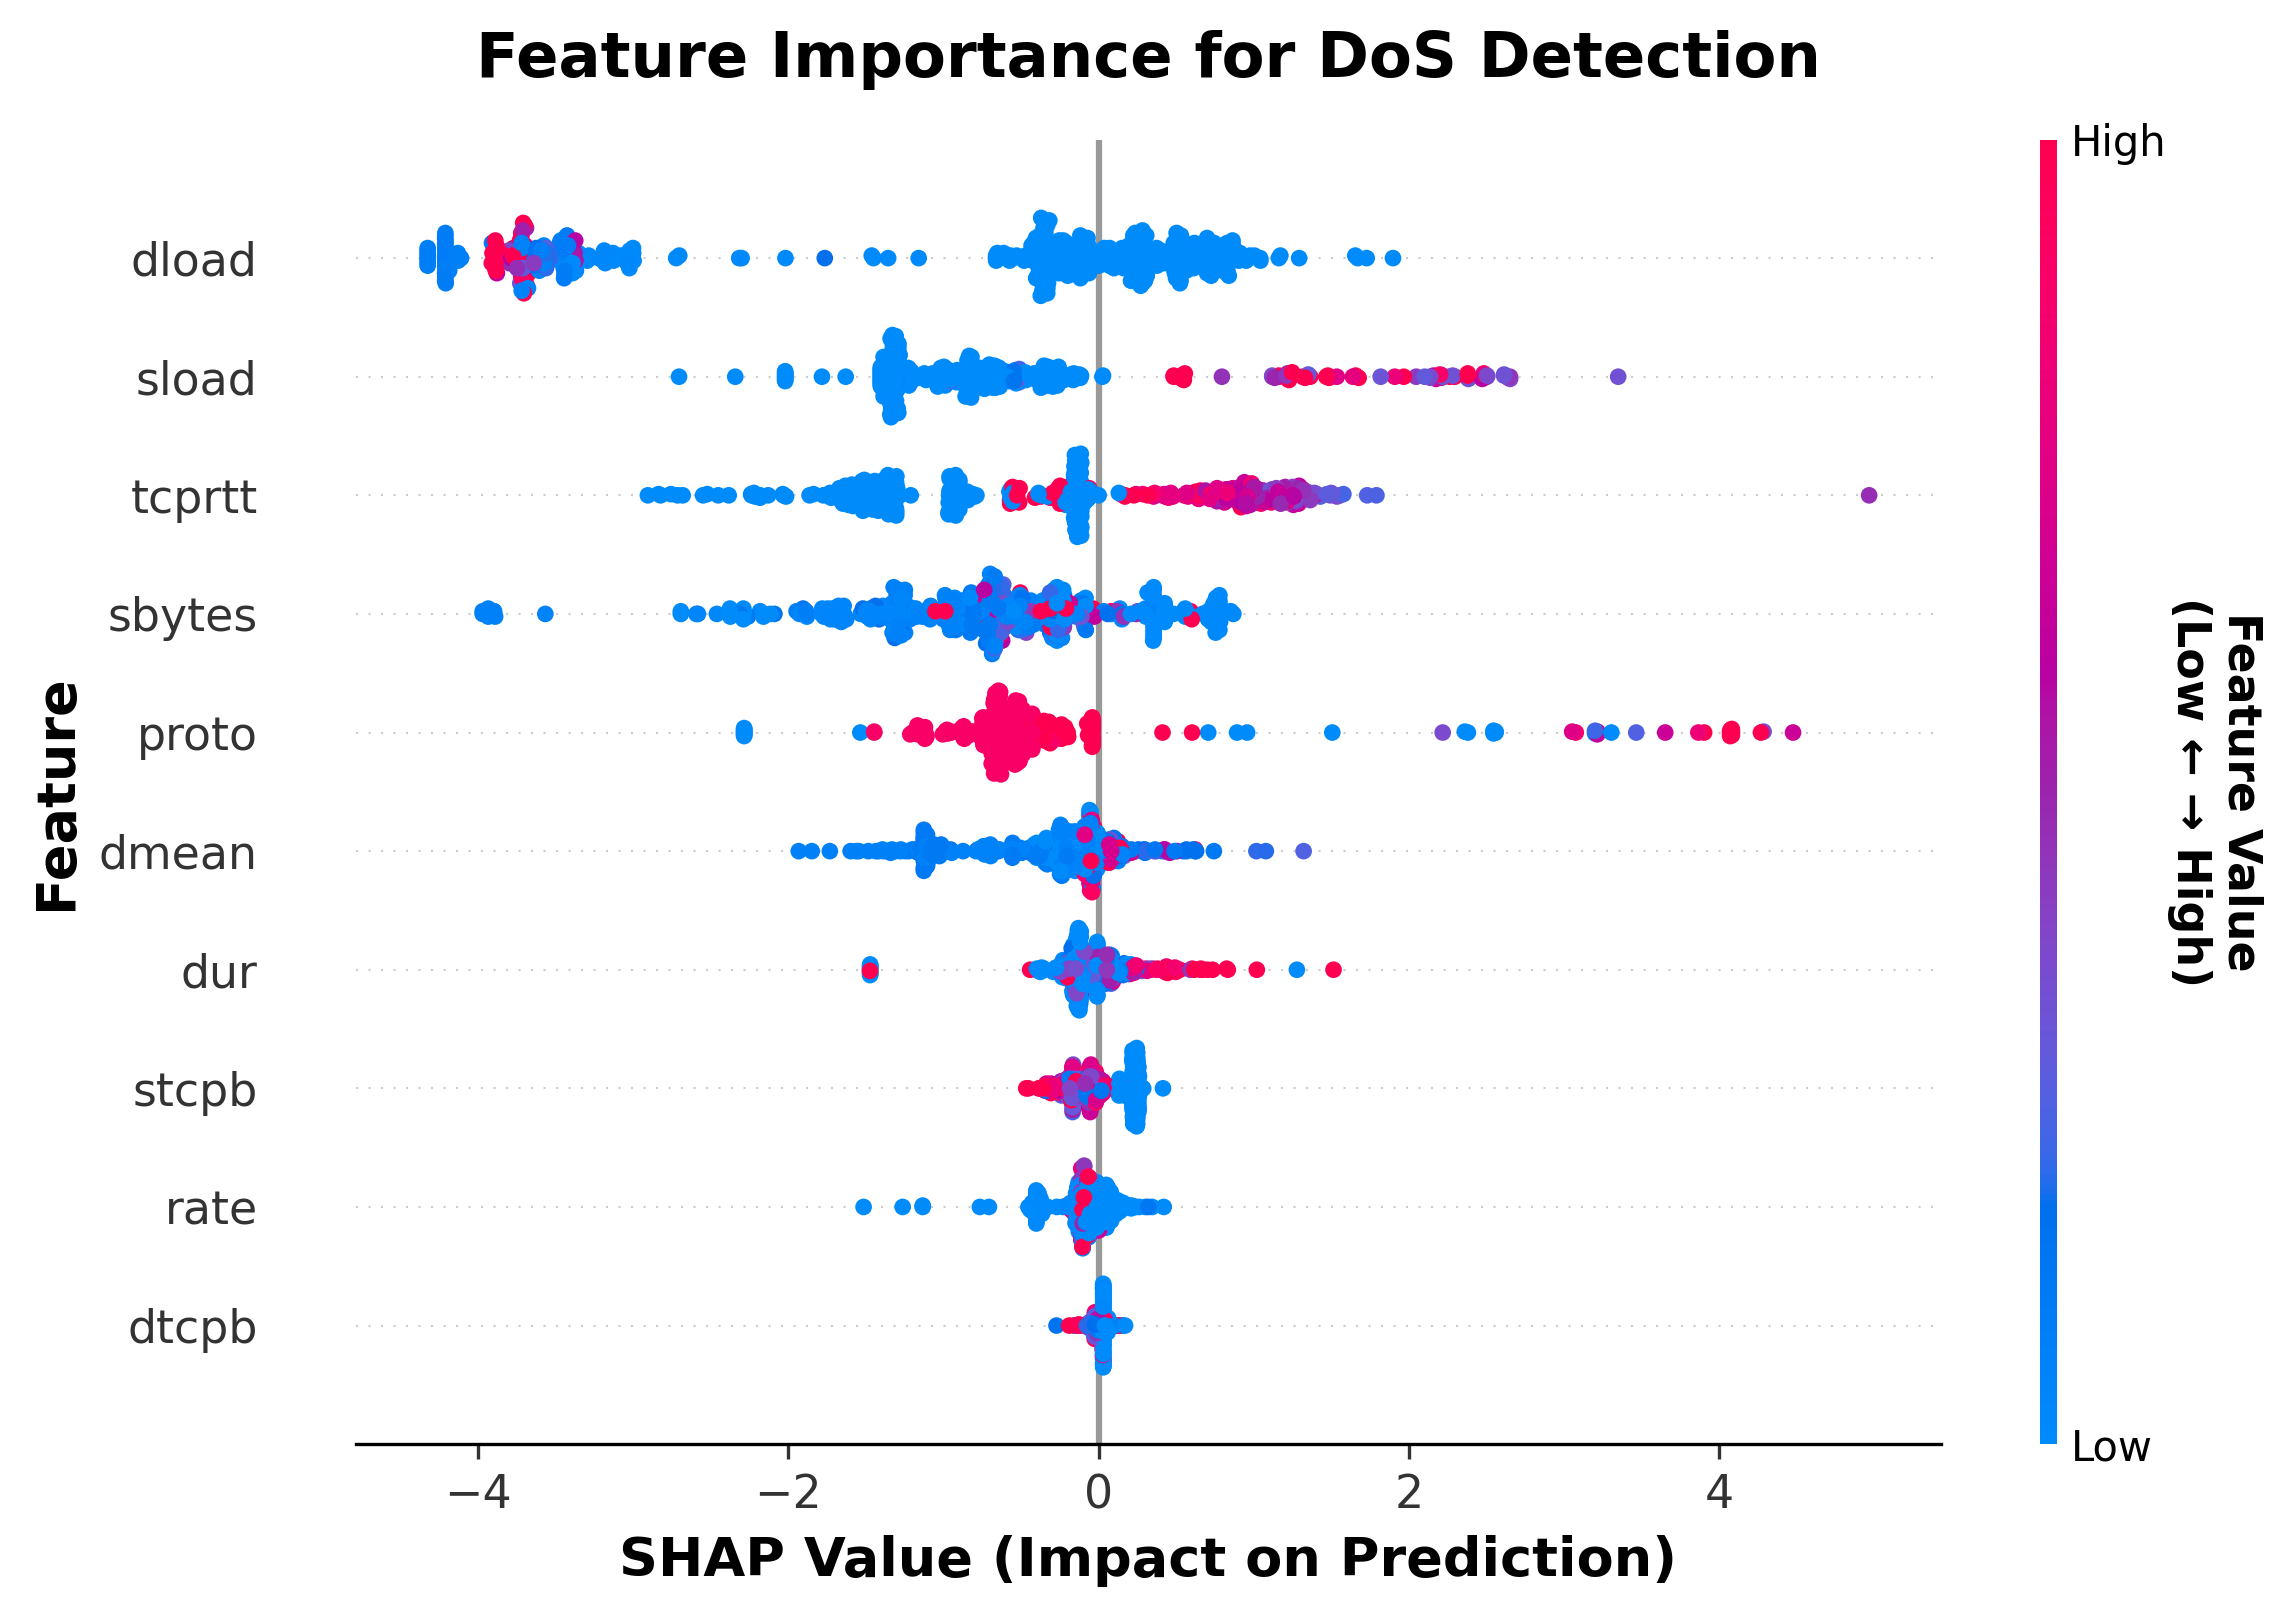
\includegraphics[width=0.85\textwidth]{04_xai_integration/images/07_shap_summary_plot.png}
    \caption{SHAP summary plot showing global feature importance across 500 samples}
    \label{fig:shap_summary}
\end{figure}

\begin{figure}[htbp]
    \centering
    \begin{subfigure}[b]{0.48\textwidth}
        \centering
        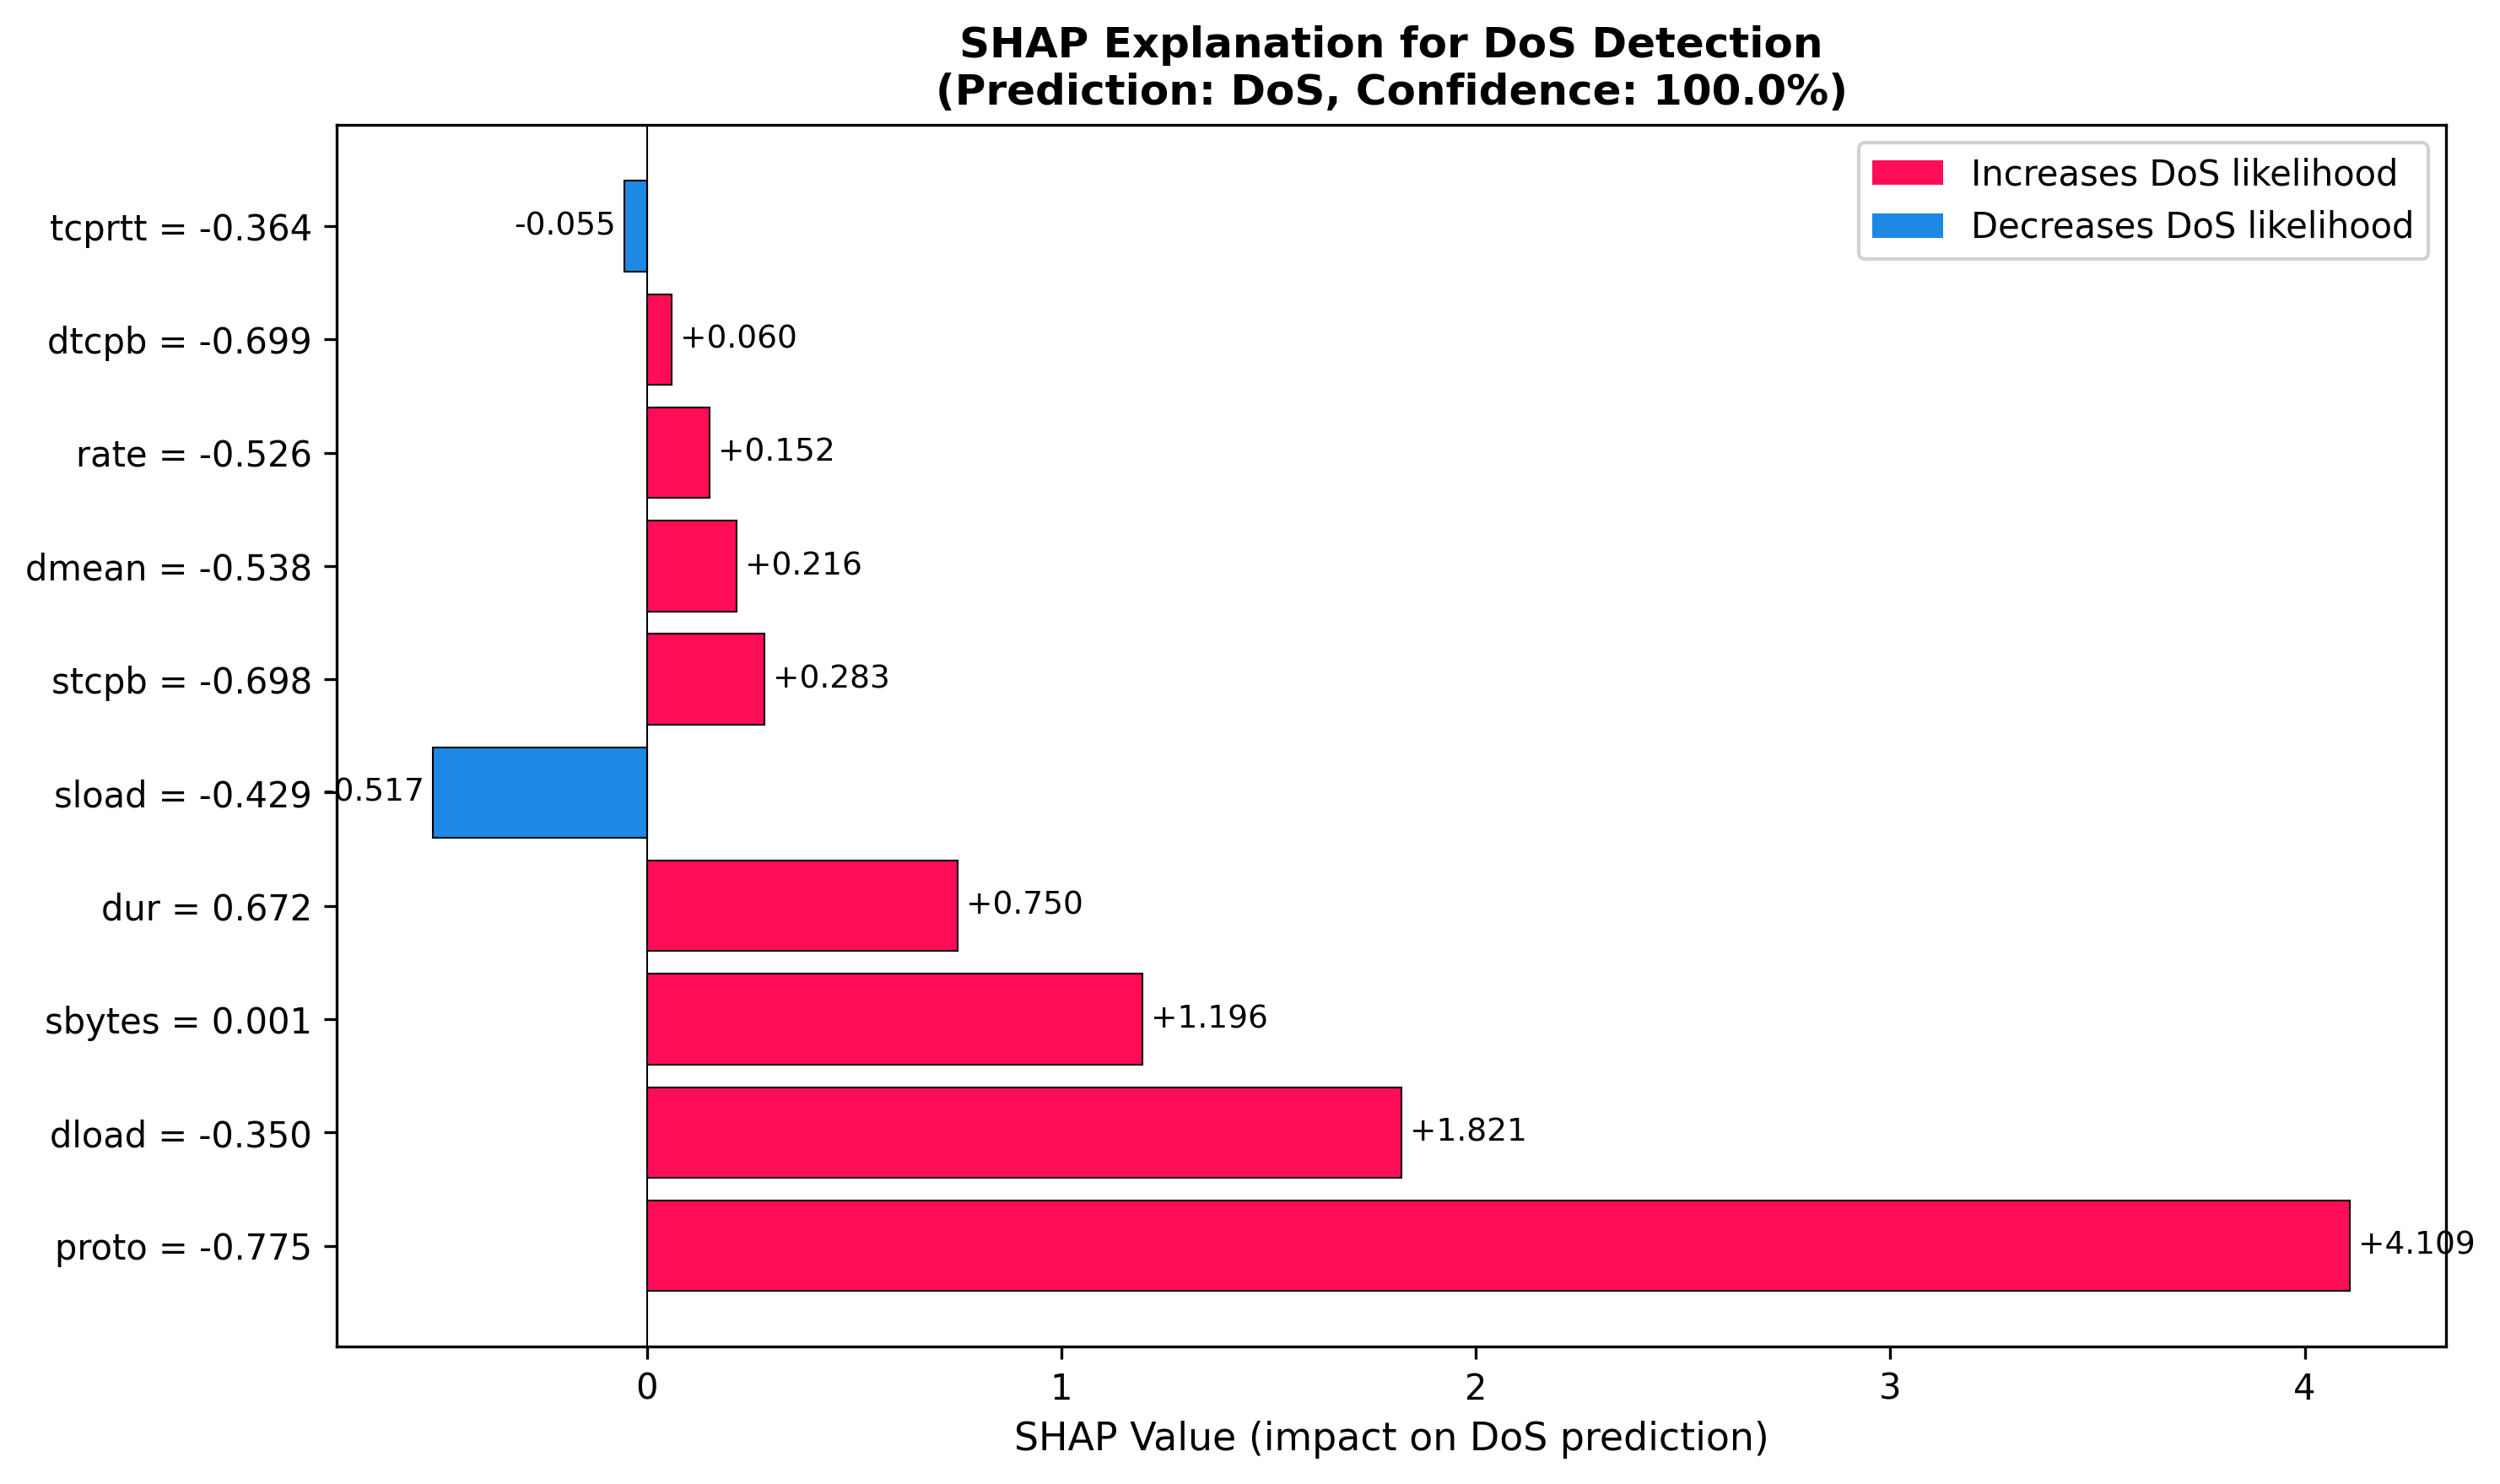
\includegraphics[width=\textwidth]{04_xai_integration/images/08_shap_waterfall_dos.png}
        \caption{DoS attack explanation}
    \end{subfigure}
    \hfill
    \begin{subfigure}[b]{0.48\textwidth}
        \centering
        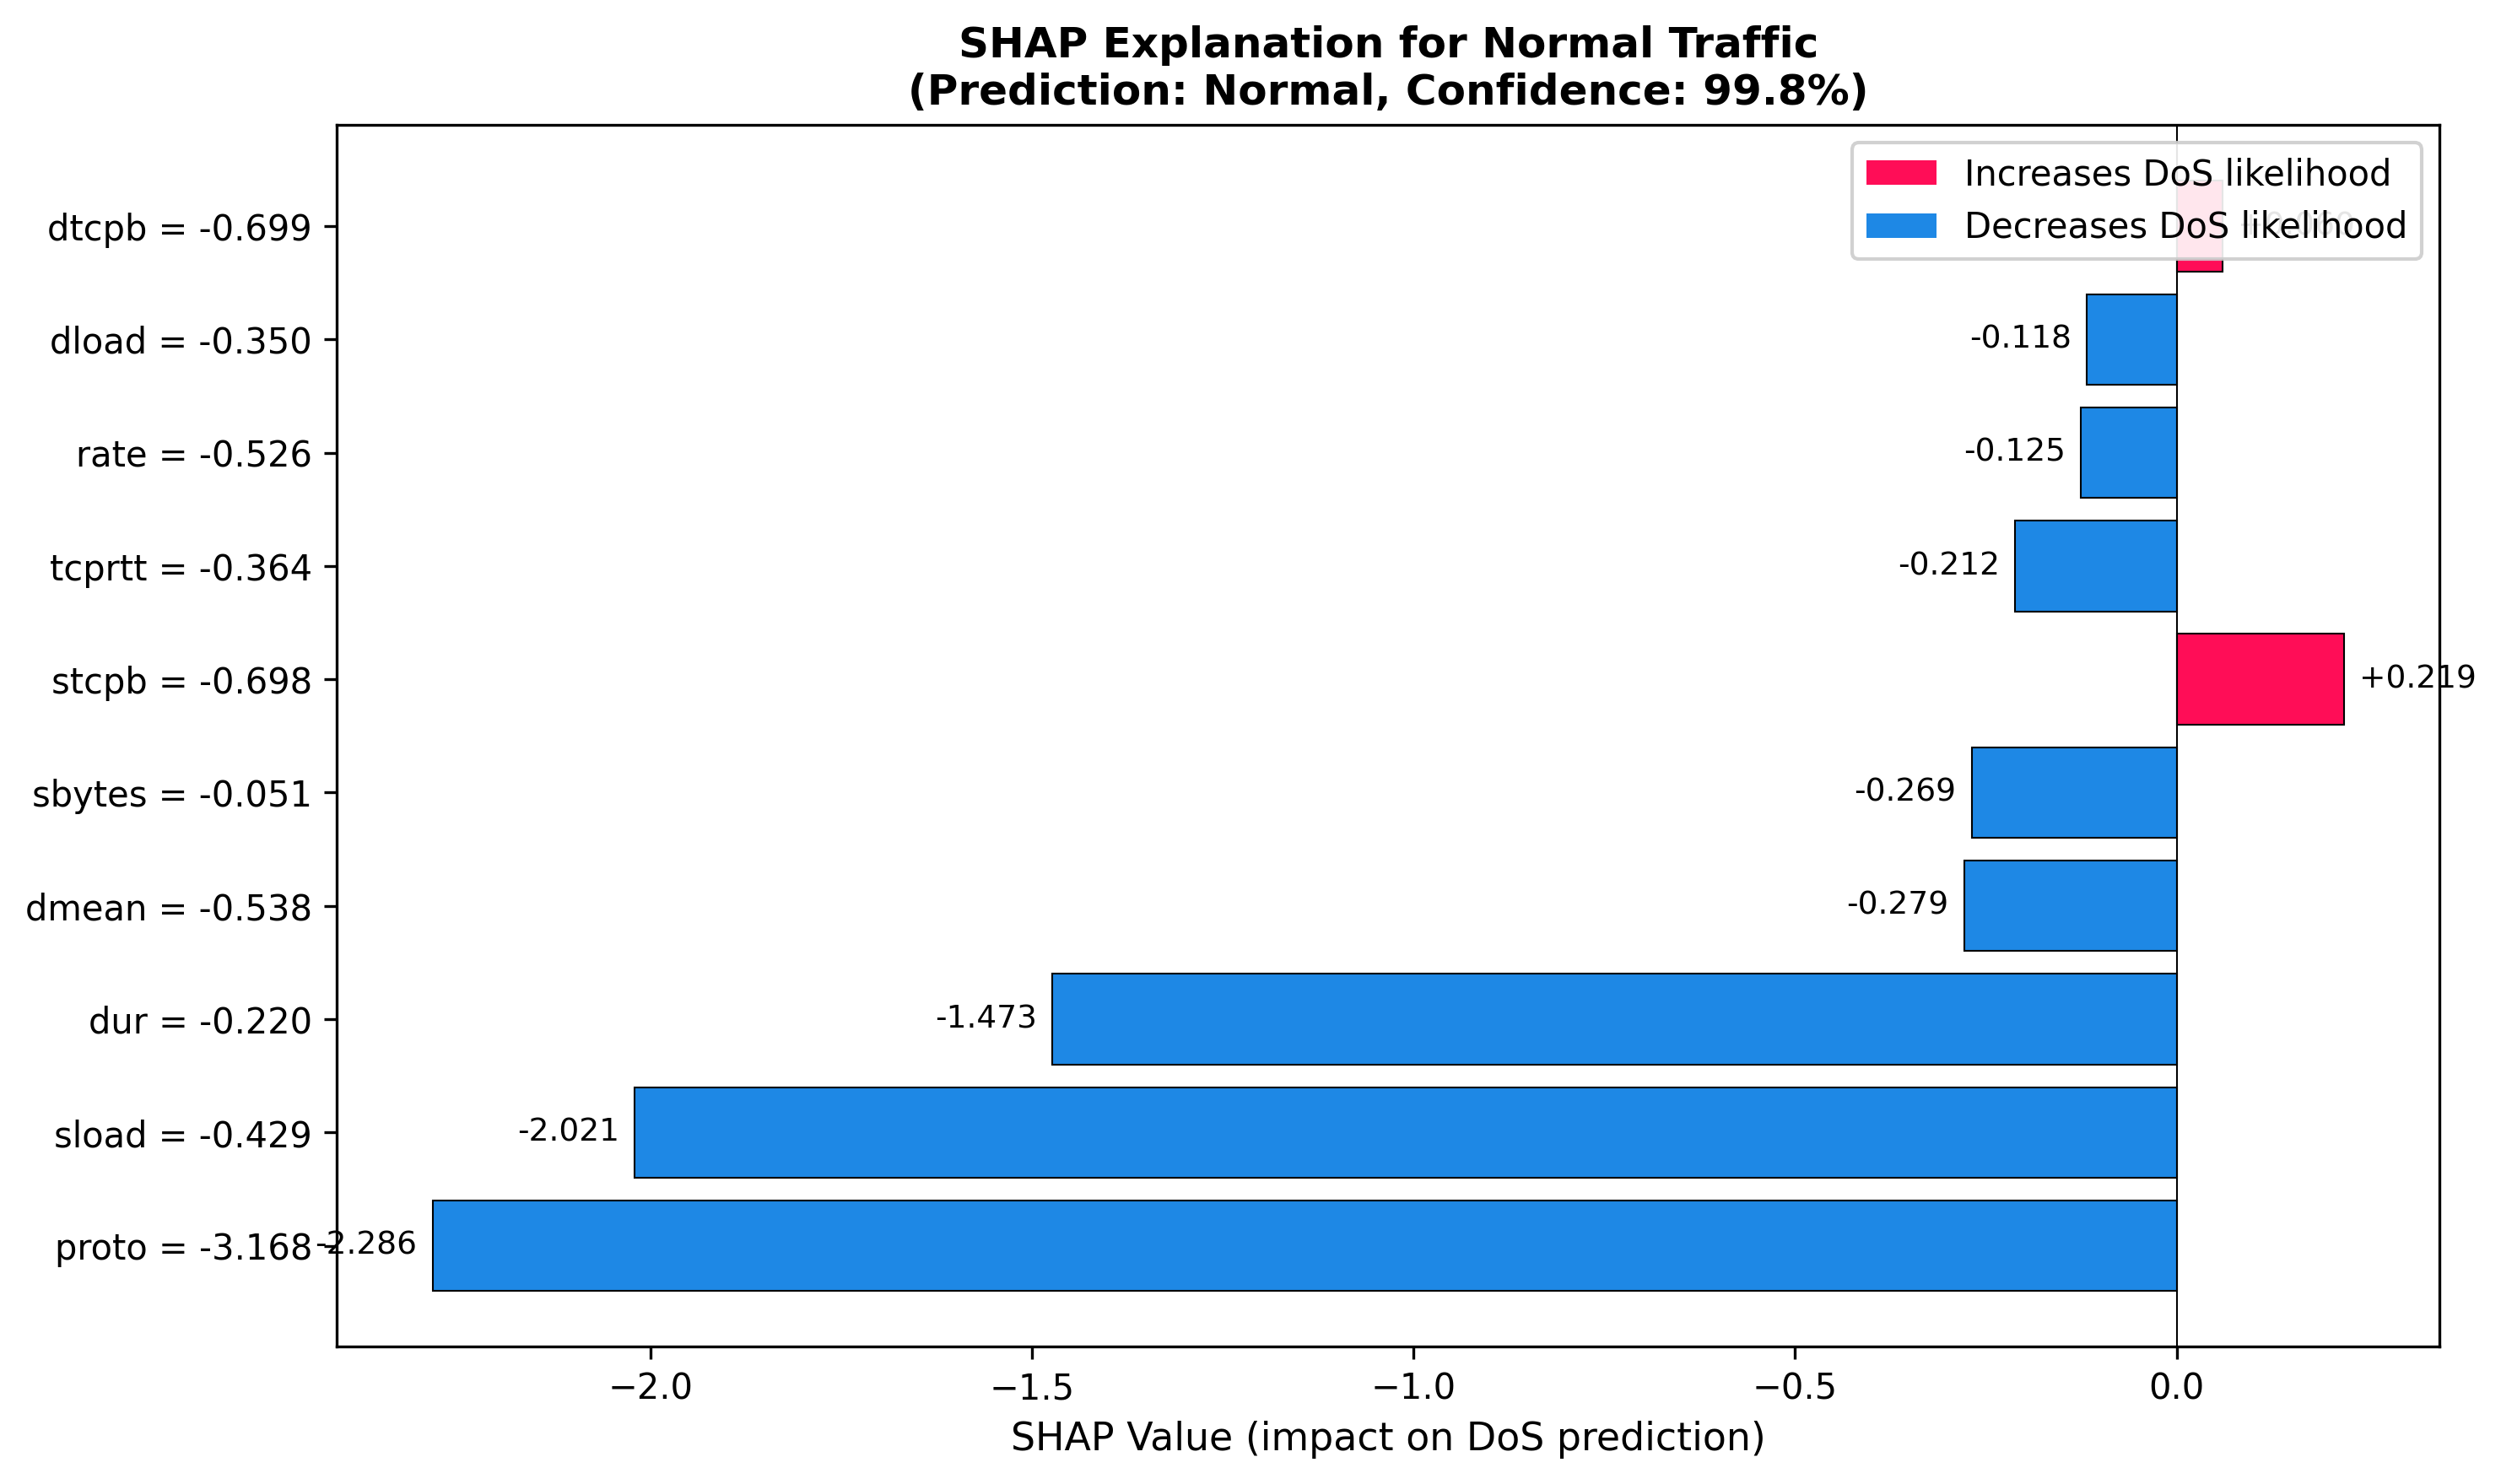
\includegraphics[width=\textwidth]{04_xai_integration/images/09_shap_waterfall_normal.png}
        \caption{Normal traffic explanation}
    \end{subfigure}
    \caption{SHAP waterfall plots for individual record explanations}
    \label{fig:shap_waterfall}
\end{figure}

\subsection{Mitigation Framework Design}

The mitigation framework represents the research novelty of this work. It converts XAI-explained detections into actionable security responses through three stages: \textit{Attack Classification}, \textit{Severity Assessment}, and \textit{Mitigation Command Generation}. The high-level design is shown in Figure~\ref{fig:mitigation_framework}.

\begin{figure}[htbp]
    \centering
    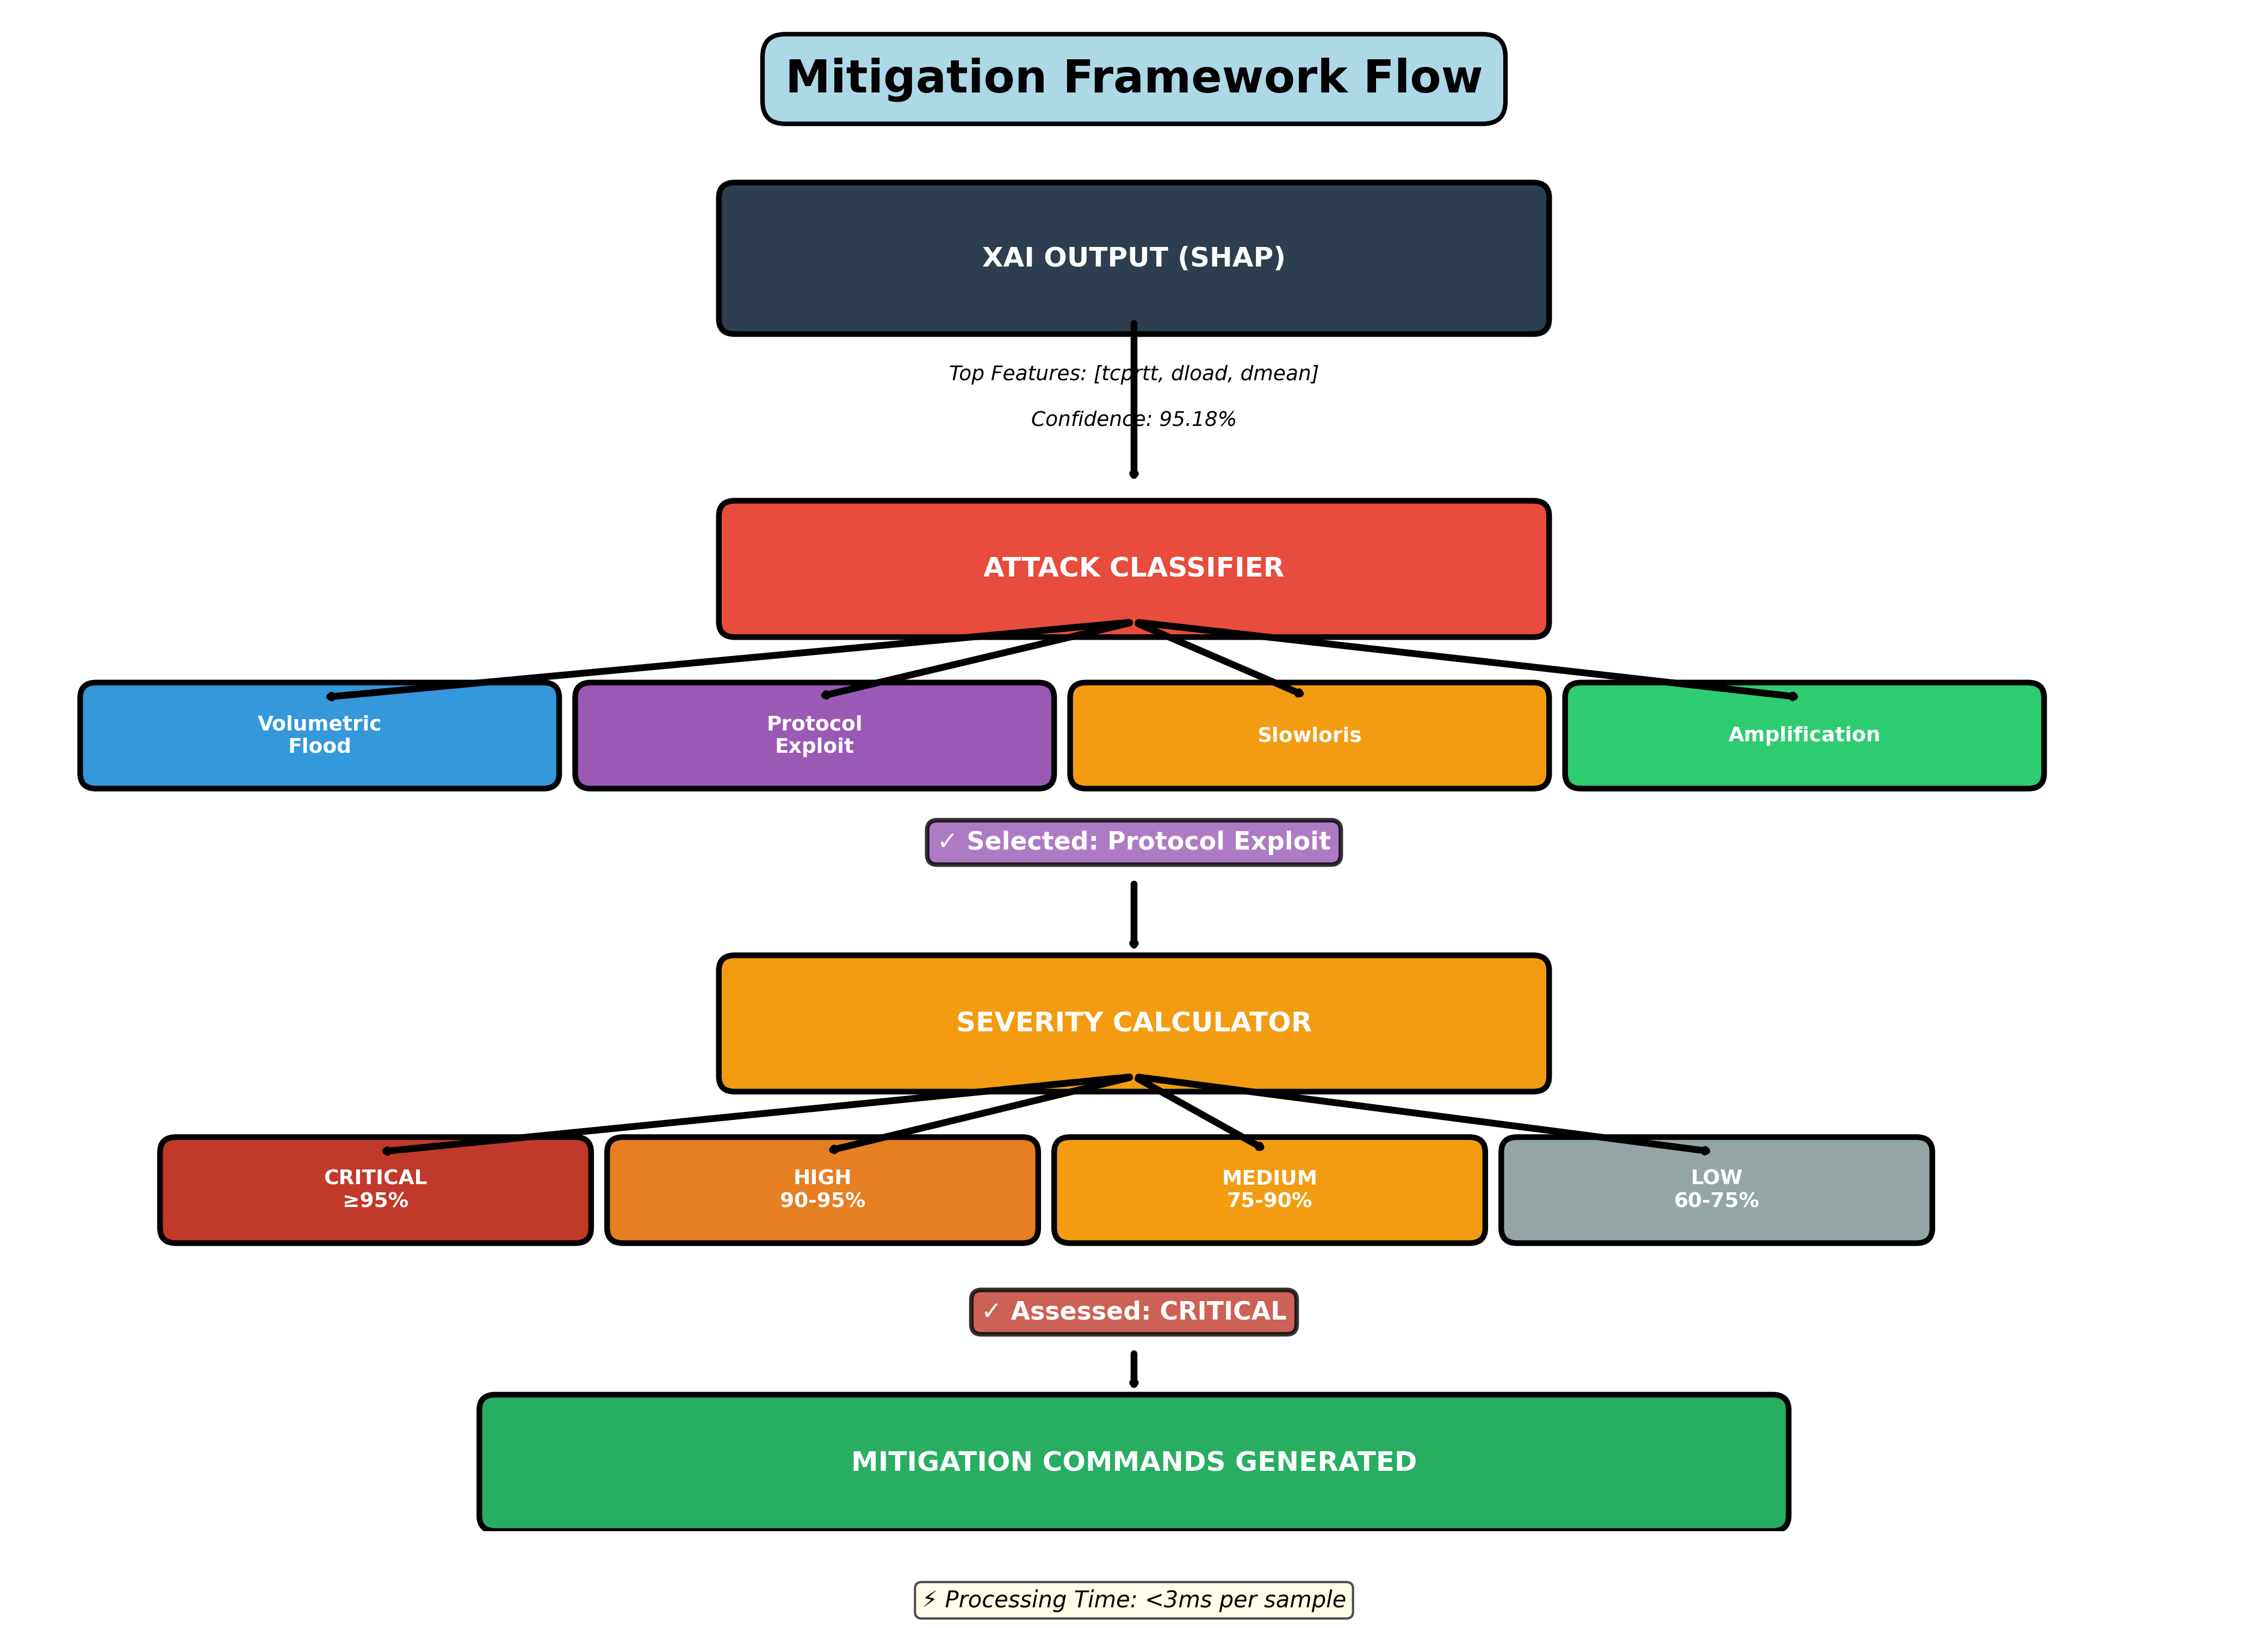
\includegraphics[width=0.90\textwidth]{presentation_diagrams/mitigation_framework_highlevel.png}
    \caption{Mitigation framework high-level design}
    \label{fig:mitigation_framework}
\end{figure}

\textbf{Attack Classification.} Based on the SHAP feature contributions and raw feature values, detected attacks are classified into four types:
\begin{enumerate}
    \item \textbf{Volumetric Flood:} Characterised by high \texttt{rate}, \texttt{sload}, and \texttt{sbytes} values (e.g., UDP flood, ICMP flood).
    \item \textbf{Protocol Exploit:} Characterised by abnormal \texttt{proto} and TCP sequence numbers (e.g., SYN flood, TCP state exhaustion).
    \item \textbf{Slowloris:} Characterised by long \texttt{dur} and low \texttt{rate} (e.g., slow HTTP attacks that hold connections open).
    \item \textbf{Amplification:} Characterised by \texttt{dload} $\gg$ \texttt{sload}, where the response is much larger than the request (e.g., DNS amplification, NTP amplification).
\end{enumerate}

\textbf{Severity Assessment.} The severity score combines three components: (1)~the model's prediction confidence as the base score, (2)~an attack type modifier (Amplification:~+15\%, Volumetric:~+10\%, Protocol:~+5\%), and (3)~a feature modifier based on extreme SHAP values (+0--10\%). The final score is mapped to four levels: CRITICAL ($\geq$95\%), HIGH (90--95\%), MEDIUM (75--90\%), and LOW (60--75\%).

\textbf{Mitigation Command Generation.} For each attack type and severity combination, the system generates specific, executable Linux commands. For example, a Volumetric Flood detection generates \texttt{iptables} rate-limiting rules and \texttt{tc} bandwidth throttling commands, while a Protocol Exploit triggers SYN cookie activation and SYN rate-limiting rules.

%----------------------------------------------------------------------
\section{Implementation Details}

\subsection{Technology Stack}

The system was implemented entirely in Python~3.x. Table~\ref{tab:tech_stack} lists the key libraries and their roles.

\begin{table}[htbp]
    \centering
    \caption{Technology stack}
    \label{tab:tech_stack}
    \begin{tabular}{lll}
        \toprule
        \textbf{Library} & \textbf{Version} & \textbf{Purpose} \\
        \midrule
        XGBoost           & 2.x   & Gradient boosting model training \\
        scikit-learn      & 1.x   & Preprocessing, cross-validation, classical models \\
        TensorFlow/Keras  & 2.x   & LSTM and 1D-CNN deep learning models \\
        SHAP              & 0.4x  & Explainable AI (TreeExplainer) \\
        Streamlit         & 1.x   & Interactive web dashboard \\
        Plotly            & 5.x   & Interactive visualisations \\
        pandas / NumPy    & ---   & Data manipulation and numerical computation \\
        \bottomrule
    \end{tabular}
\end{table}

\subsection{Project Structure}

The project is organised into modular directories, each corresponding to a research objective:

\begin{itemize}
    \item \texttt{01\_data\_preparation/} --- Raw dataset storage and initial data loading scripts.
    \item \texttt{03\_model\_training/proper\_training/} --- Model training scripts, saved models (\texttt{.pkl}, \texttt{.keras}), saved preprocessors (scaler, encoder), and generated evaluation images.
    \item \texttt{04\_xai\_integration/} --- SHAP TreeExplainer wrapper class (\texttt{shap\_explainer.py}), test scripts, and SHAP visualisation images.
    \item \texttt{05\_mitigation\_framework/} --- Attack classifier (\texttt{attack\_classifier.py}), severity calculator (\texttt{severity\_calculator.py}), mitigation command generator (\texttt{mitigation\_generator.py}), and alert generator (\texttt{alert\_generator.py}).
    \item \texttt{06\_complete\_testing/} --- Full pipeline benchmark test scripts and result visualisations.
    \item \texttt{dashboard.py} --- Standalone Streamlit dashboard integrating the entire pipeline.
\end{itemize}

\subsection{Dashboard Implementation}

An interactive Streamlit web dashboard was developed to provide a user-friendly interface for the complete detection pipeline. The dashboard allows users to:
\begin{itemize}
    \item Upload CSV files containing network traffic records (supporting both UNSW-NB15 and CIC-IDS2017/CIC-DDoS2019 formats via an automatic adapter).
    \item View real-time detection results with colour-coded severity indicators.
    \item Inspect per-record SHAP explanations through interactive waterfall plots.
    \item Review attack type classifications and severity assessments.
    \item Copy generated mitigation commands for immediate deployment.
\end{itemize}

The dashboard loads the saved XGBoost model, StandardScaler, and LabelEncoder at startup and processes uploaded records through the full pipeline: preprocessing $\rightarrow$ detection $\rightarrow$ SHAP explanation $\rightarrow$ attack classification $\rightarrow$ severity assessment $\rightarrow$ mitigation command generation.

%----------------------------------------------------------------------
\section{Prototype \& Testing}

\subsection{Full Pipeline Benchmark}

The complete end-to-end pipeline was tested on all 41,089~official benchmark samples from the UNSW-NB15 external testing set. The results confirm that the integrated system maintains the same detection performance as the standalone model while successfully generating explanations, attack classifications, severity levels, and mitigation commands for every detected attack. Table~\ref{tab:benchmark_results} summarises the final benchmark results, and Figure~\ref{fig:pipeline_diagram} illustrates the complete pipeline flow.

\begin{table}[htbp]
    \centering
    \caption{Full pipeline benchmark results (41,089 samples)}
    \label{tab:benchmark_results}
    \begin{tabular}{lc}
        \toprule
        \textbf{Metric} & \textbf{Value} \\
        \midrule
        Accuracy         & 98.14\% \\
        Precision        & 94.42\% \\
        Recall           & 86.45\% \\
        F1 Score         & 90.26\% \\
        AUC              & 0.9915  \\
        False Alarm Rate & 0.56\% (209 / 37,000) \\
        Processing Rate  & 422.1 samples/second \\
        Processing Time  & 1.62 minutes (all 41,089 samples) \\
        \bottomrule
    \end{tabular}
\end{table}

\begin{figure}[htbp]
    \centering
    \includegraphics[width=0.90\textwidth]{06_complete_testing/pipeline_flow_diagram.png}
    \caption{Complete pipeline flow diagram}
    \label{fig:pipeline_diagram}
\end{figure}

\subsection{Confusion Matrix Analysis}

The confusion matrix for the full pipeline test (Figure~\ref{fig:cm_heatmap}) reveals that 36,791 out of 37,000~normal samples were correctly identified (99.44\% specificity), with only 209~false positives. On the attack side, 3,535 out of 4,089~DoS attacks were correctly detected (86.45\% recall), with 554~attacks missed. This represents an operationally acceptable trade-off: the system maintains an extremely low false alarm rate while detecting the vast majority of attacks.

\begin{figure}[htbp]
    \centering
    \includegraphics[width=0.60\textwidth]{06_complete_testing/confusion_matrix_heatmap.png}
    \caption{Full pipeline confusion matrix heatmap}
    \label{fig:cm_heatmap}
\end{figure}

\subsection{Attack Classification and Severity Distribution}

When the 3,744 detected attack records (3,535~TP + 209~FP) were processed through the mitigation framework, the attack type distribution (Figure~\ref{fig:attack_dist}) shows that Volumetric Floods constitute 81.3\% of detections, followed by Protocol Exploits at 17.6\%, Amplification at 1.0\%, and Slowloris at 0.1\%. This distribution is consistent with the known characteristics of the UNSW-NB15 dataset, which predominantly contains high-volume flooding attacks.

The severity distribution shows that 99.97\% of detections were classified as CRITICAL and 0.03\% as HIGH, reflecting the high confidence of the XGBoost model on correctly detected attacks.

\begin{figure}[htbp]
    \centering
    \begin{subfigure}[b]{0.48\textwidth}
        \centering
        \includegraphics[width=\textwidth]{06_complete_testing/attack_type_distribution.png}
        \caption{Attack type distribution}
    \end{subfigure}
    \hfill
    \begin{subfigure}[b]{0.48\textwidth}
        \centering
        \includegraphics[width=\textwidth]{06_complete_testing/severity_distribution.png}
        \caption{Severity level distribution}
    \end{subfigure}
    \caption{Distribution of attack types and severity levels across all detections}
    \label{fig:attack_dist}
\end{figure}

\subsection{Comparison with Literature}

Table~\ref{tab:literature_comparison} compares the evaluation methodology of this work against common practices in intrusion detection literature. While many published works report F1~scores above 95\%, these are typically achieved on balanced test sets with same-dataset splits. The results in this study, evaluated on an imbalanced external test set, provide a more rigorous and realistic assessment of model performance.

\begin{table}[htbp]
    \centering
    \caption{Comparison of evaluation methodology with common literature practices}
    \label{tab:literature_comparison}
    \begin{tabular}{lll}
        \toprule
        \textbf{Aspect} & \textbf{Common Practice} & \textbf{Our Approach} \\
        \midrule
        Test Set Balance     & Balanced (50/50)             & Imbalanced (90/10) \\
        Validation Type      & Same dataset split           & External dataset (separate CSV) \\
        Reported Metrics     & Accuracy, F1 only            & Full metrics + AUC + CM \\
        Typical F1 Reported  & 95\%+                        & 90.57\% \\
        Realistic?           & No (inflated)                & \textbf{Yes} (honest evaluation) \\
        \bottomrule
    \end{tabular}
\end{table}
